\documentclass[a4paper]{article}
\usepackage{geometry}
\geometry{margin=1in}

\usepackage[english]{babel}
\usepackage[utf8]{inputenc}
\usepackage{amsmath}
\usepackage{graphicx}
\usepackage[colorinlistoftodos]{todonotes}
\usepackage{gensymb}
\usepackage{hyperref}
\usepackage[T1]{fontenc}
\usepackage{lmodern}
\usepackage{minted}
\usepackage{url}
\usepackage{fancyhdr}
\usepackage{wrapfig}

\setlength{\parskip}{0.7em}
\setlength{\parindent}{0in}

\title{ \textbf{Introduction to Programming \& The Internet of Things} \\
Module 2: Introduction to Arduino \vspace{-5ex} \\
}
\date{}

\begin{document}
\maketitle
\thispagestyle{fancy}
\lhead{University of Texas at Austin \\ Civil, Architectural, and Environmental Engineering \\ Material curated by Thomas Dougherty}
\rhead{Professor Dr. Zoltan Nagy \\ https://nagy.caee.utexas.edu \\ Fall 2018}

\section{Modules Background}
There is a pervasive need to study the performance of built structures and their abilities to provide occupants with comfort in an efficient manner. The Internet of Things (IoT) provides methods of obtaining and studying data about our built environments. As such, these modules introduce civil, architectural, and environmental engineers to tropics of electrical engineering. Students will gather the abilities needed to program and deploy necessary sensors in the Internet of Things (IoT), as well as gain the ability to gather and analyze data collected.

\tableofcontents
\newpage

\section{Introduction}
\label{sec:introduction}

Alright!! Time to build some little robots. This little computer called the \textbf{Arduino} will allow us to read and interact with sensors, motors, other computers, you name it! Once you master a few basics, collecting data and building robots will be entirely possible. Let's jump in!

\section{Getting Started with Arduino}
\label{fig:arduino}
\begin{wrapfigure}{r}{0.5\textwidth}
  \begin{center}
    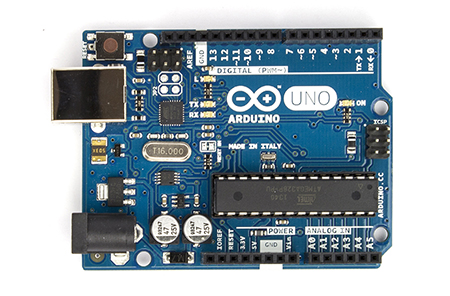
\includegraphics[width=0.5\textwidth]{1-6.jpg}
  \end{center}
  \caption{Ardunio Uno}
\end{wrapfigure}
\label{sec:starting}
First, let's check out the hardware. Our lovely little board has a lot going on, so this first section will be discussing its capabilities.

To give you visual clues and help you follow along this tutorial, I'll be using the online Arduino simulator \cite{tinkercad} which you can follow to validate that your electronic design and code are appropriate. Without further ado, let's jump in!

\subsection{Power}
There are a few different ways to power our little board. We can use the silver rectangular block (top left of fig 1) to plug in a USB cable, we can use the black DC power jack (bottom left of fig 1), or we can plug into the VIN and GND pins. Our wee board accepts a range of 7-12V through the DC jack and input pins, and 5V through the usb (although you won't need to think of this very often). For this module, we'll just be using the USB.

\subsection{Pins}
On the board you'll find 14 digital I/O \cite{gpio} pins. These are labeled as 0-13. These are used to tell if a voltage is high or low. We'll get into that more later. Likewise, you'll also find that 6 of these pins also provide PWM \cite{pwm} output which can give you "analog output". The pins that are capable of producing PWM signals are labeled with "\~{}".

You'll also find that the board contains 6 analog input pins. These are labeled as A0-A5. These are truly analog, and they allow us to measure a range of voltages from 0-5V. These values are mapped to a range of numbers from 0-1023, so our precision is 0.0049V and our max speed is 10,000 samples per second. Good enough for government work (Just kidding, it may not be. Please don't use this value if you're building high precision laser systems or something wild later).

\section{Code}
\subsection{Arduino IDE}
The Arduino platform \cite{arduino_software} was chosen for these modules in large part because of their accessibility, ease of use, and free software. It contains all of the software you'll need, with support for every platform. It is \textbf{highly} recommended that you download the software if you would like to work within the Ardunio platform.

\begin{figure}
\centering
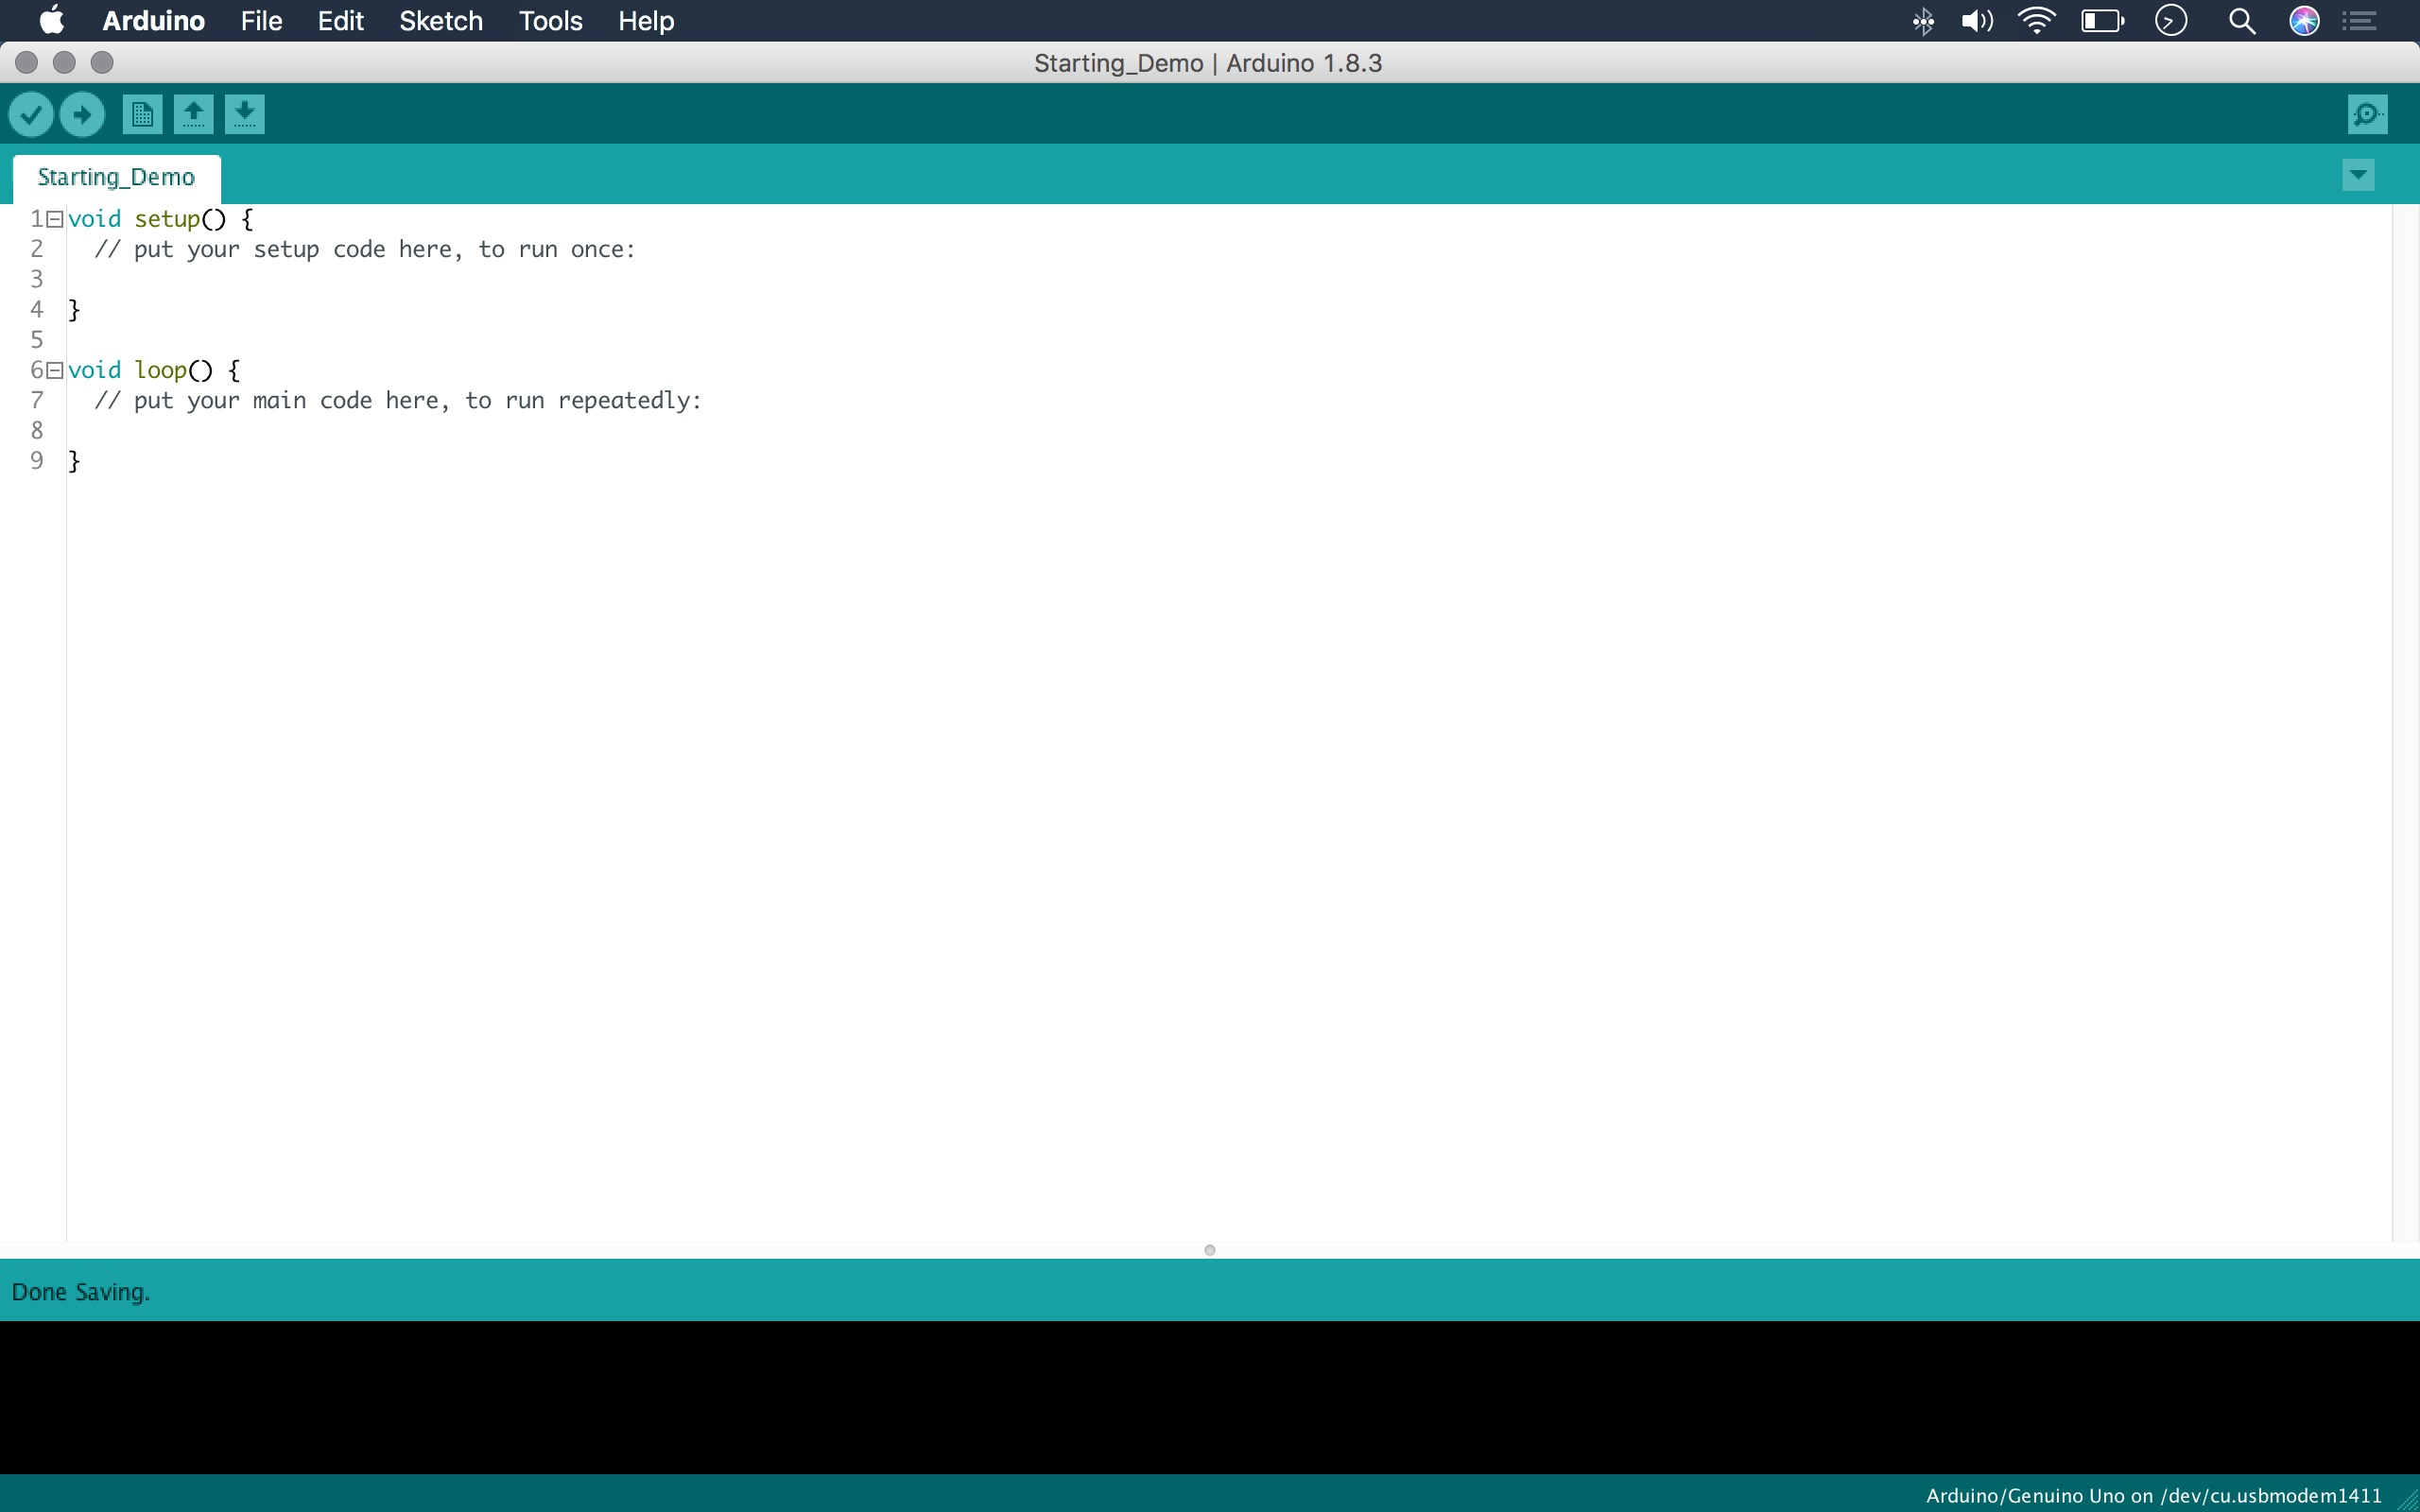
\includegraphics[width=1\textwidth]{1-7.jpg}
\caption{\label{fig:arduino_ide}Arduino IDE}
\end{figure}

\subsection{Basics}
We're going to start with the basic "blink" sketch, something to toggle a light going on and off. To follow the process of the computer, think about the logic it must follow. Thinking about the most essential functions it has to accomplish, it needs to know a couple of things: if it's going to push high voltage or read voltage levels (in or out), and where this pushing and pulling will happen.

This requires that we tell the computer which pin we'd like to use. Normally, it's convenient to define the pin at the beginning before the setup so that it can be easily changed if needed later. In this case, the variable my\_pin will always reference the number 13. If at a later point we change the 13 to say 10, we won't need to change every instance of the number 13 in the rest of the code.

\subsubsection{Digital Out}

\begin{minted}{c++}
int my_pin = 13;
\end{minted}

Now to tell the computer we'd like to use this pin, we use this syntax:

\begin{minted}{c++}
pinMode(my_pin, OUTPUT);
\end{minted}

Where again, the variable "my\_pin" could be replaced with the number 13 as well. This step usually goes in the "setup" function, which is \underline{only run once}.

To tell this pin if we'd like it to push high or low, we pass this command:
\begin{minted}{c++}
digitalWrite(my_pin, HIGH);
\end{minted}
or
\begin{minted}{c++}
digitalWrite(my_pin, LOW);
\end{minted}

This normally goes in the "loop()" function, which runs \underline{indefinitely}. If we want to make an oscillating high and low signal, we might do something like this:

\begin{minted}{c++}
void loop()
{
  // turn the LED on (HIGH is the voltage level)
  digitalWrite(my_pin, HIGH);
  delay(100); // Wait for 100 millisecond(s)
  // turn the LED off by making the voltage LOW
  digitalWrite(my_pin, LOW);
  delay(100); // Wait for 100 millisecond(s)
}
\end{minted}

Using this code with a 200-1000 (1k) Ohm resistor and an LED, you'll see that the LED begins to blink!

\subsubsection{PMW - "Analog" Output}

\begin{figure}
\centering
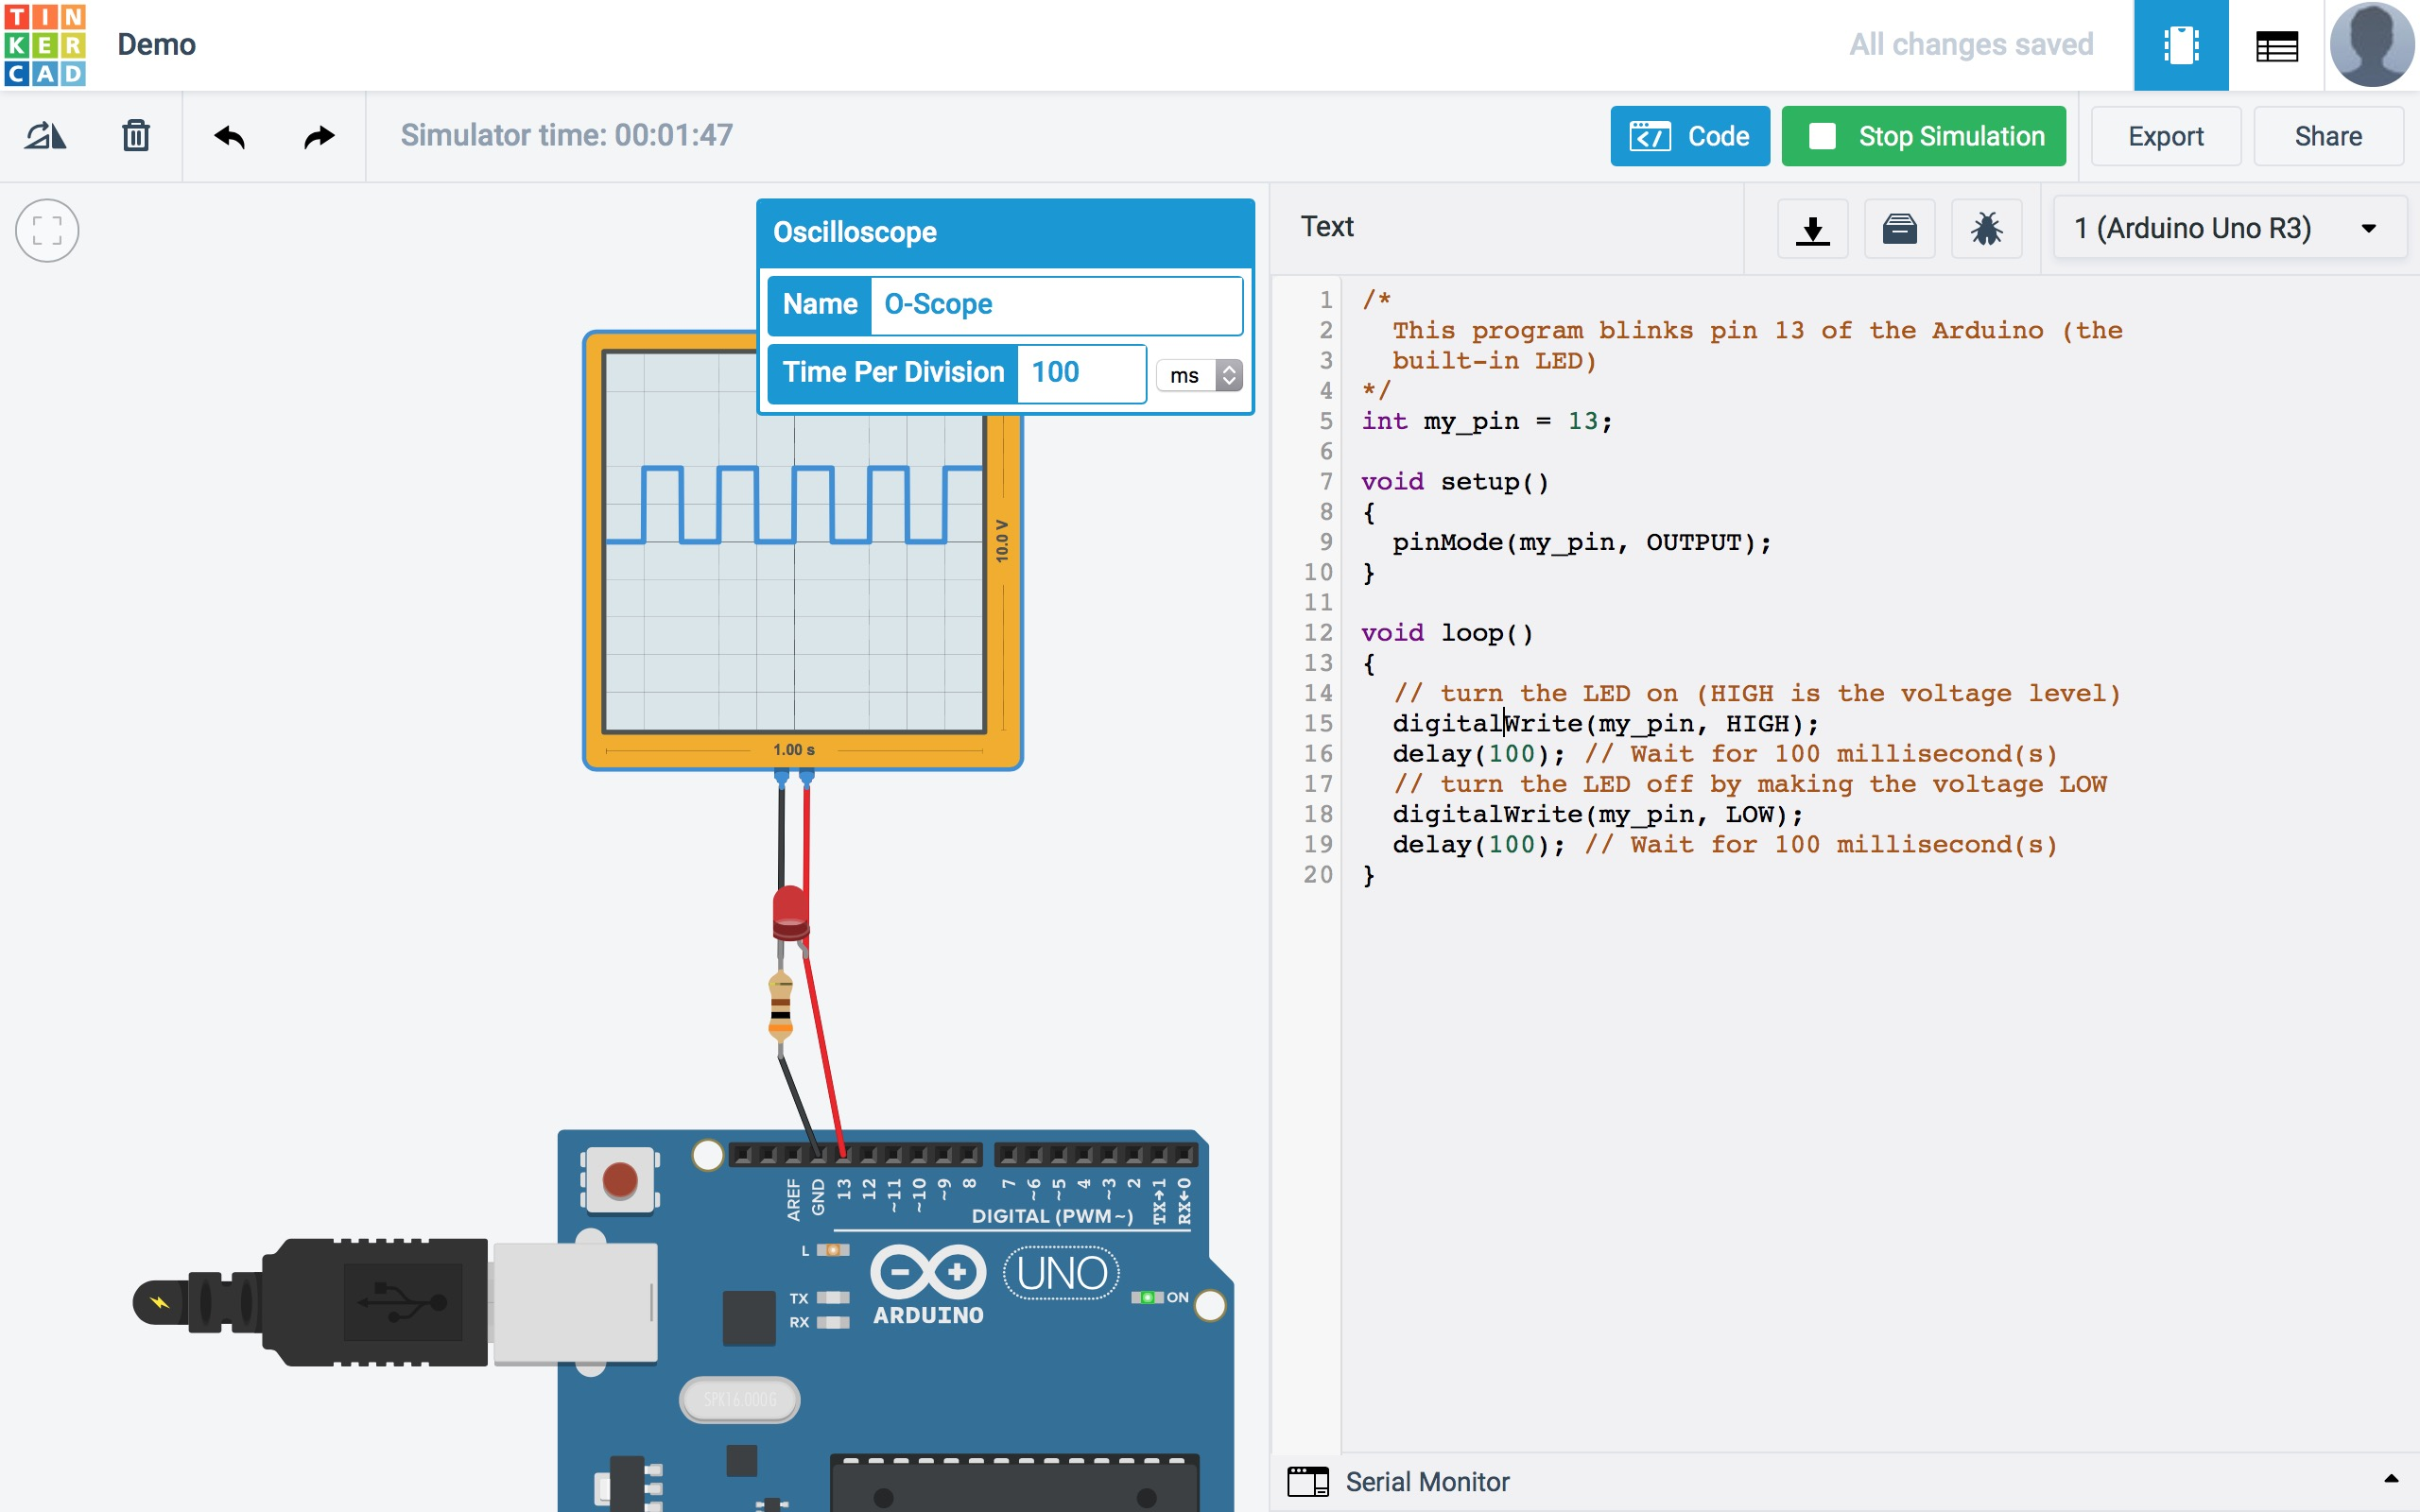
\includegraphics[width=1\textwidth]{1-3.jpg}
\caption{\label{fig:arduino_ide}Arduino Blink}
\end{figure}

PWM tricks your eyes into perceiving an analog output by modifying what percentage of the time the value in coming in as on. For example, an led being powered by a PWM signal of 80\% might look like it is in reality receiving 80\% of the brightness of a "fully" on LED. See \cite{ardunio_pwm} if you'd like more information about PWM.

To use it with the Arduino, we initialize it the same was as the digital write function. We then call it like this:
\begin{minted}{c++}
void loop(){
analogWrite(10,200);
}
\end{minted}
Two things to note:
\begin{enumerate}
\item Only the pins with the \~{} are capable of producing PWM outputs. On the Arduino Uno, these pins are 3,5,6,9,10, and 11.
\item While the first number in the \textbf{analogWrite} function designates the pin number, the second is the "analog" output value. This range only goes from 0 to 255, with 255 being the maximum voltage output (or the same as digitalWrite(13, HIGH)).
\end{enumerate}

\subsubsection{Digital Input}
Next, we need to be able to read if a value is high or low. To do this, we'll change the syntax just a wee bit. Instead of writing the pinMode as OUTPUT, we want to define it as an INPUT. The resulting code in the setup function will look like this instead:

\begin{figure}
\centering
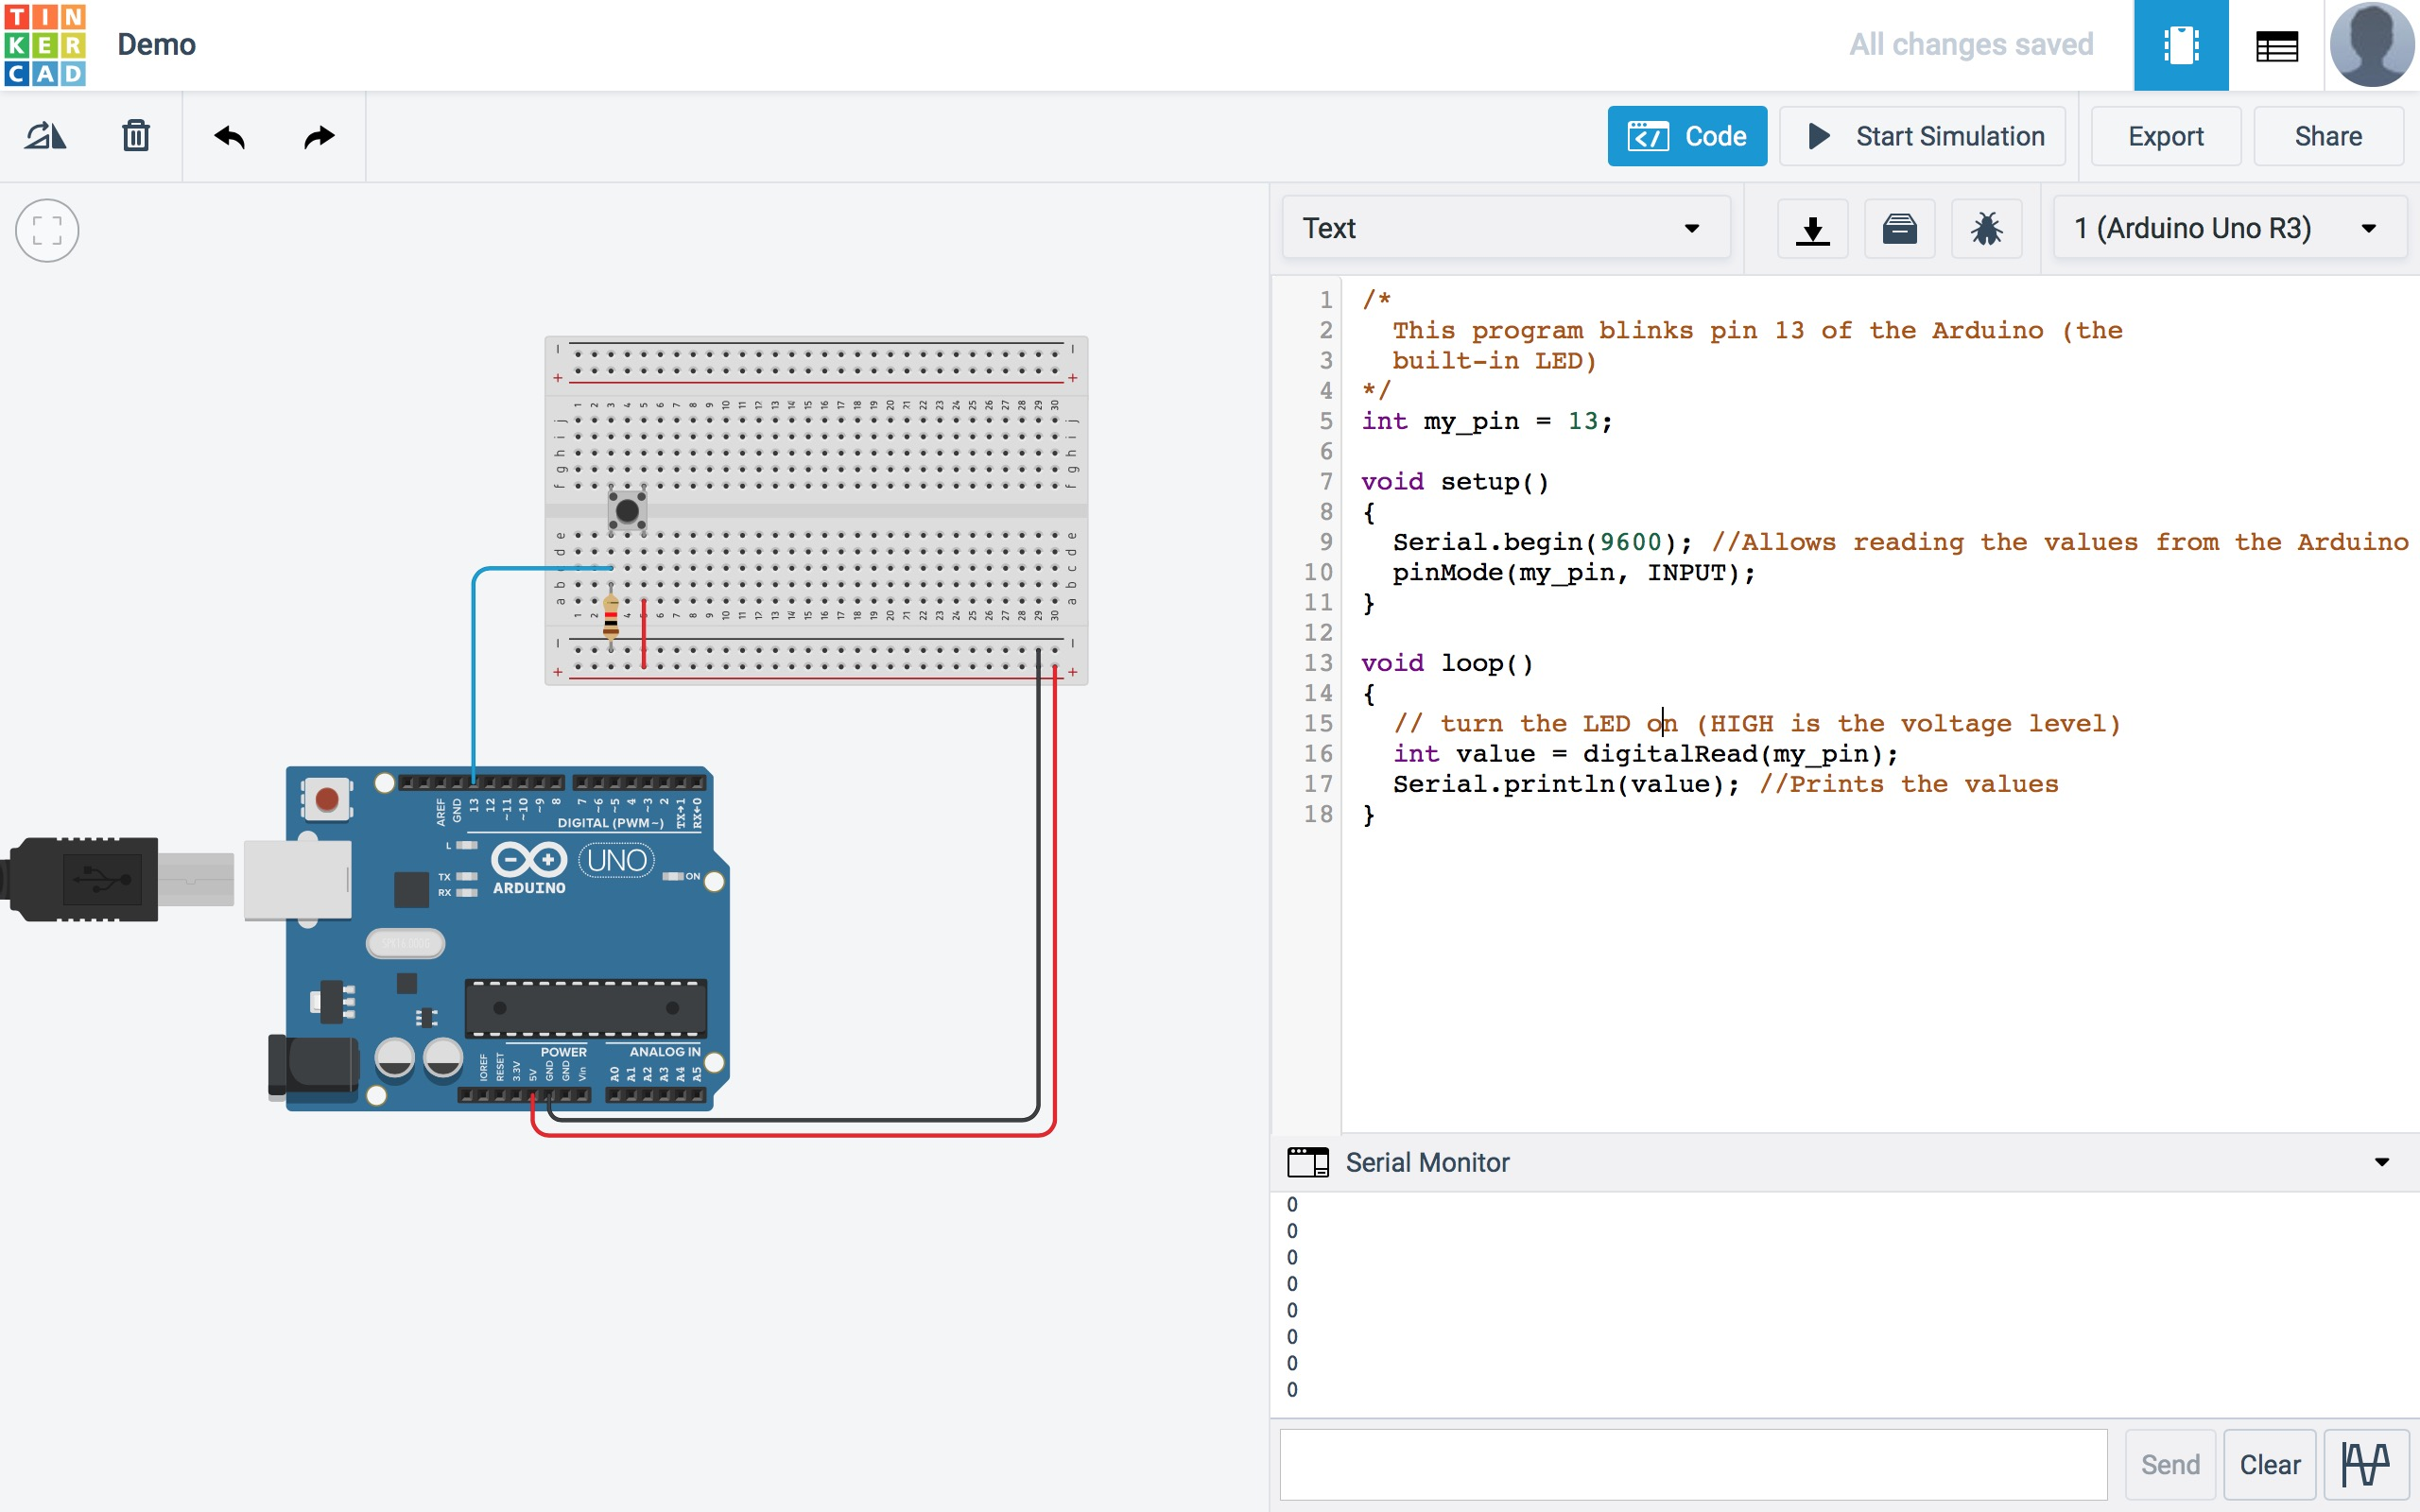
\includegraphics[width=1\textwidth]{1-4.jpg}
\caption{\label{fig:button}Button}
\end{figure}

Notice a couple of things. There's a command called \textbf{digitalRead}, which returns a value which must be a number. The example stored this as a variable called "value".

Also take note of the hardware setup. The use of a resistor connected to GND acts as a kind of dam, keeping the computer from shorting itself by connecting GND directly to 5V every time the button is pushed. The pin we're using to read the voltage is still upstream of this button, so it can "feel" the effect of high voltage when the button is pressed and connected to the 5V terminal.

Final note for this image, notice the use of a \textbf{Serial} command. The Serial monitor allows information to be sent through the USB cable and onto the computer, allowing for real time analysis and debugging. To use it, copy the example code's setup process and printing system. Then just replace the data you'd like to see with the "value" term that's filling it in the example.

\subsubsection{Analog Input}
The Arduino supports up to 6 analog inputs, but they require special pins. These are the pins named A0-A5. To use them, we'll need to define our pin like this:

\begin{minted}{c++}
void setup(){
pinMode(A0, INPUT);
}
\end{minted}
and use them like this:
\begin{minted}{c++}
void loop(){
int my_var = analogRead(A0);
}
\end{minted}
where "A0" can be any of the analog input terminals. See the Figure \ref{fig:analog_in} for wiring to a photoresistor.


\begin{figure}
\centering
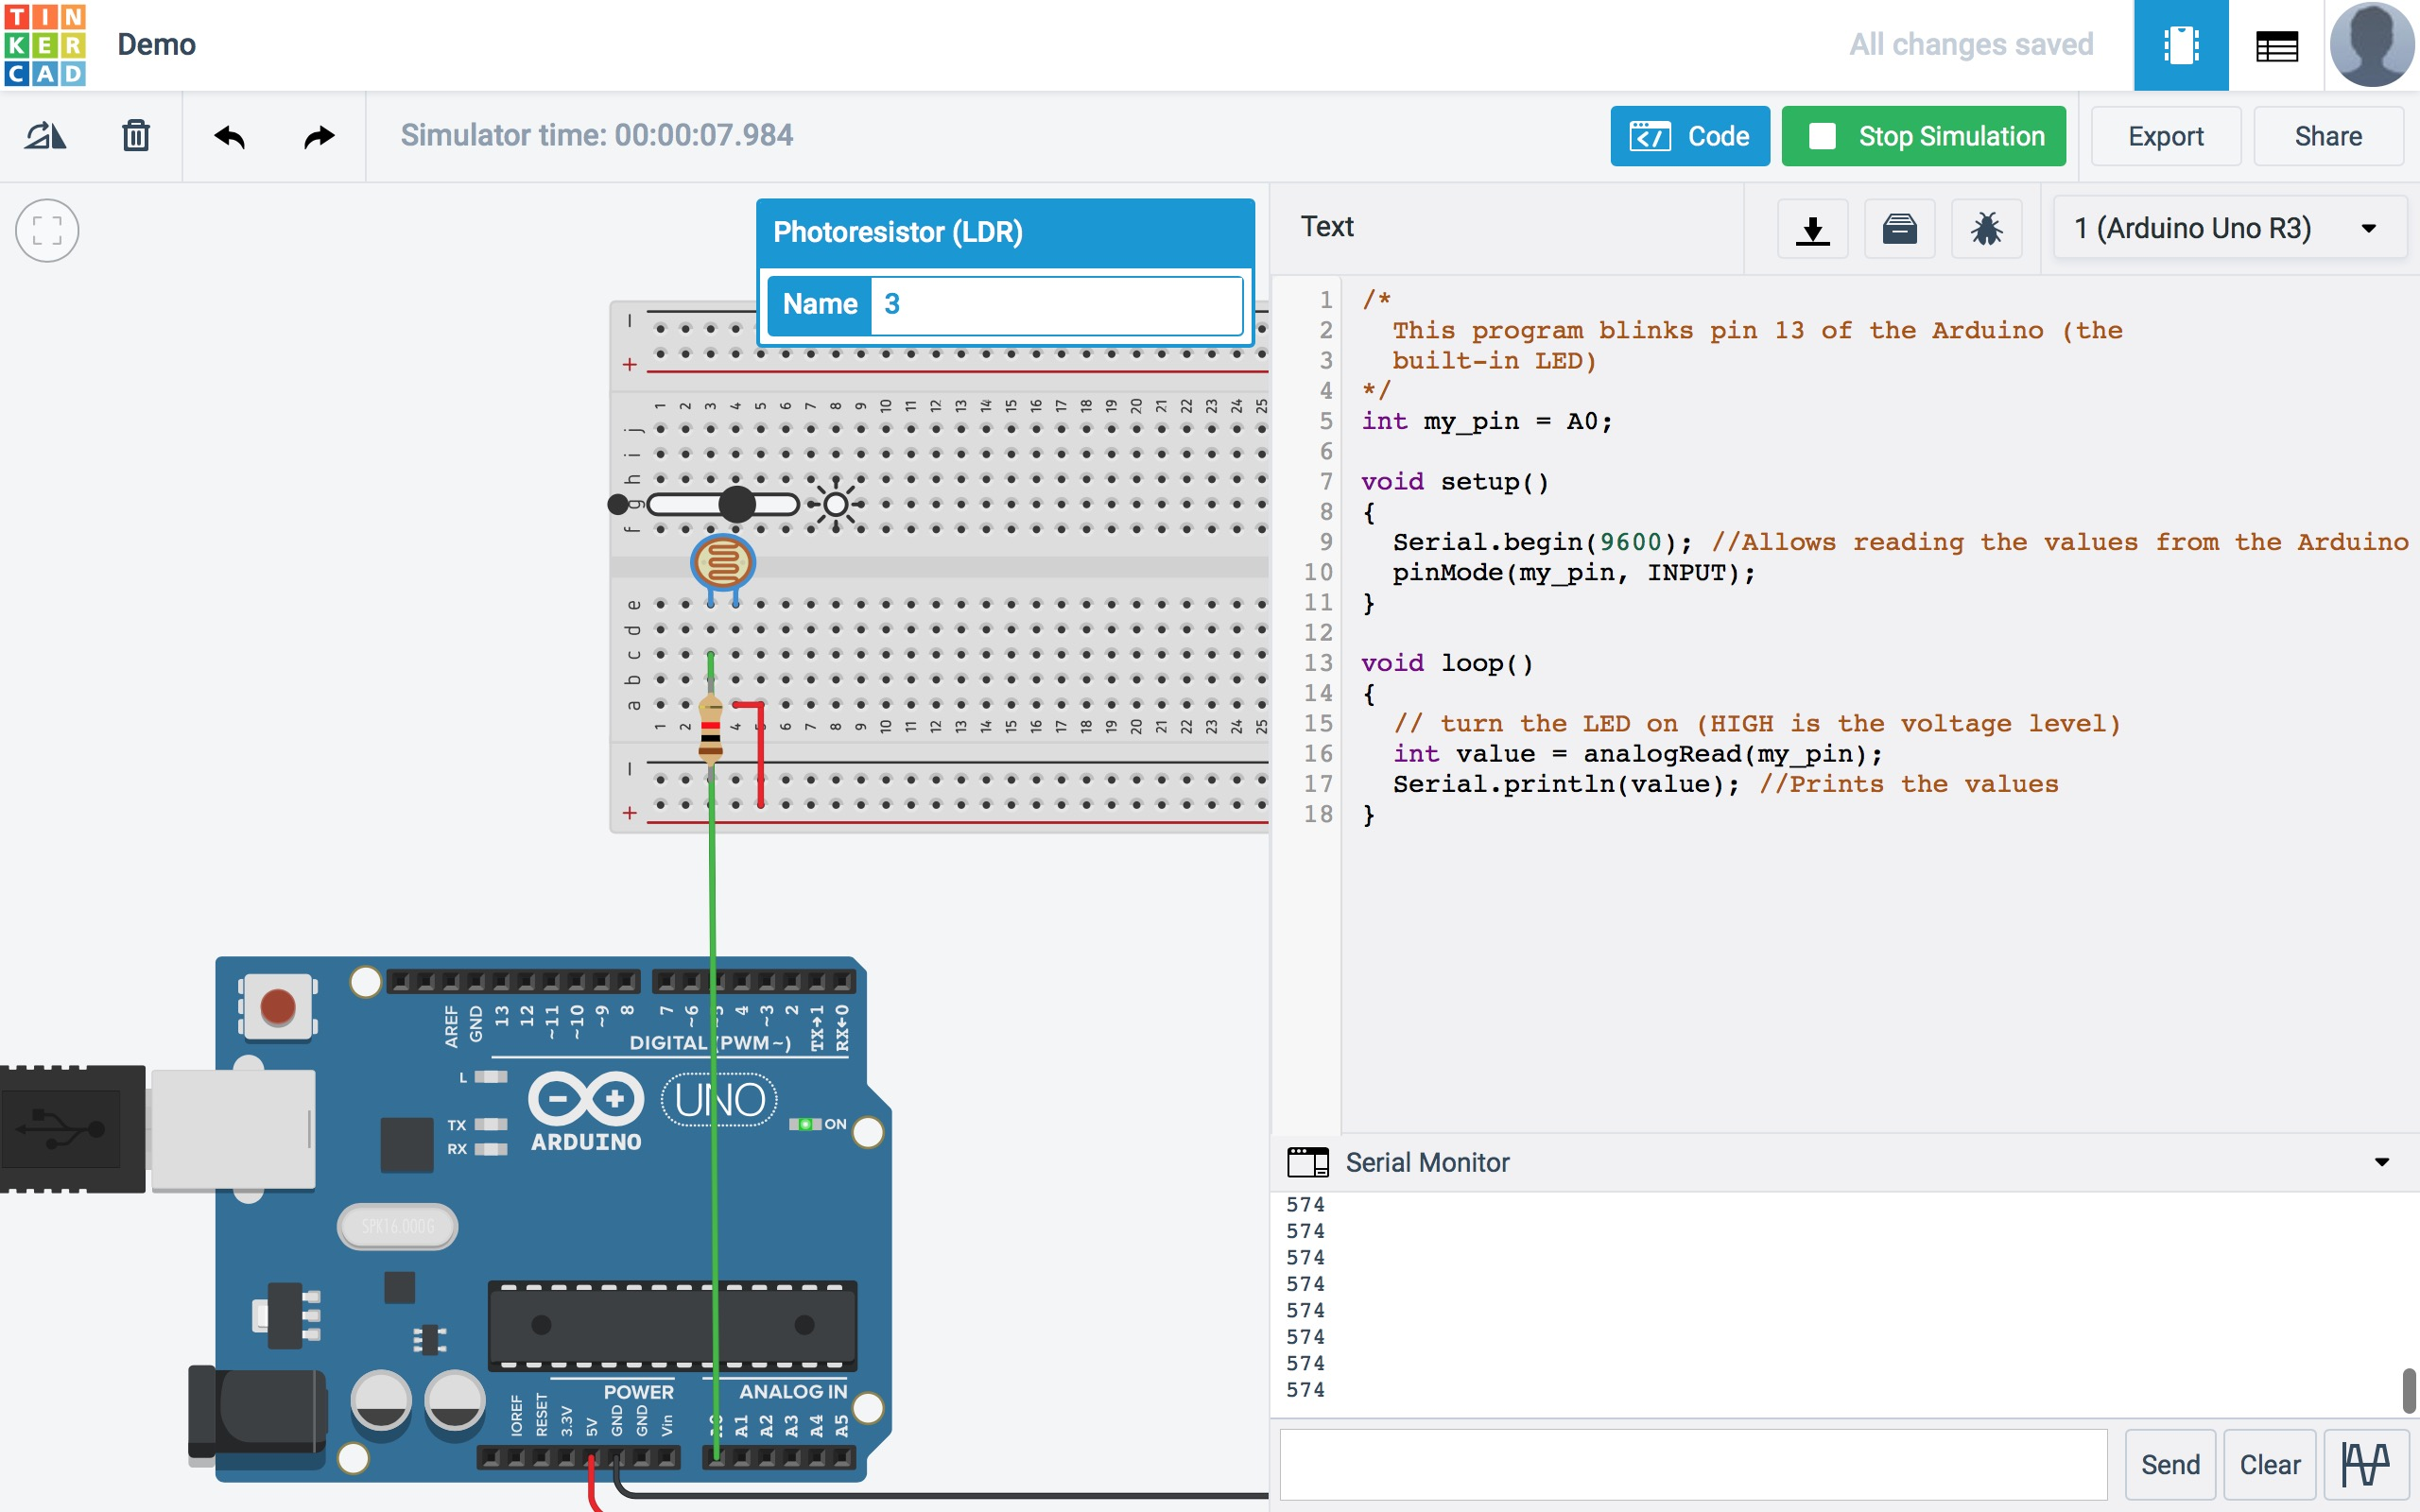
\includegraphics[width=1\textwidth]{1-2.jpg}
\caption{\label{fig:analog_in}Analog In.}
\end{figure}

\newpage
\section{Exercises}
Q1 -  Build an array of lights (maybe three in a row) that sequentially change from dark to bright.
\newline
Q2 -  Turn on a light \textbf{if} a button is pressed.
\newline
Q3 -  Turn on a light \textbf{if} it's dark.
\newline
Q4 -  Make a button that adds to a counter every time it's pressed.
\newline
Q5 -  Use the systems you built in problems 1 and 4 to make a new system that sequentially lights up LEDs if a button is pressed. 

\bibliographystyle{unsrt}
\bibliography{references.bib}

\end{document}